\documentclass[12pt]{article}

\usepackage{amsmath,amssymb}
\usepackage{graphicx}

\usepackage{setspace}
\onehalfspacing
\usepackage[margin=1in]{geometry}
\usepackage{hyperref}
\hypersetup{allcolors=blue, colorlinks=true}
\usepackage[utf8]{inputenc}
% Notation
% Mathematical functions
\newcommand{\isone}[1]{{\boldsymbol{1}\left( #1 \right)}}
\renewcommand{\Pr}[1]{{\mathbb{P}\left(#1\right) }}
\newcommand{\f}[1]{{f\left(#1\right) }}
\newcommand{\Prcond}[2]{{\mbox{Pr}\left(#1\vphantom{#2}\;\right|\left.\vphantom{#1}#2\right)}}
\newcommand{\fcond}[2]{{f\left(#1|#2\right) }}
\newcommand{\Expected}[1]{{\mathbb{E}\left\{#1\right\}}}
\newcommand{\ExpectedCond}[2]{{\mathbb{E}\left\{#1\vphantom{#2}\;\right|\left.\vphantom{#1}#2\right\}}}

\newcommand{\Likelihood}[2]{\text{L}\left(#1 \left|\vphantom{#1}#2\right.\right)}
\newcommand{\sufstats}[1]{s\left(#1\right)}
\renewcommand{\exp}[1]{\mbox{exp}\left\{#1\right\}}
\newcommand{\transpose}[1]{{#1}^\mathbf{t}}

% Objects
\newcommand{\params}{\theta}
\newcommand{\Params}{\Theta}
\newcommand{\Graph}{\mathbf{G}}
\newcommand{\graph}{\mathbf{g}}
\newcommand{\GRAPH}{\mathcal{G}}
\newcommand{\Adjmat}{Y}
\newcommand{\adjmat}{y}
\newcommand{\ADJMAT}{\mathcal{Y}}

\newcommand{\INDEPVAR}{\mathcal{X}}
\newcommand{\Indepvar}{X}
\newcommand{\indepvar}{x}

\newcommand{\normconst}{\kappa\left(\params, \Indepvar\right)}

% \graphicspath{{./fig/}}


%% NEED THIS FOR CANCY TEX
\usepackage{pstricks}

% Colors
\definecolor{USCCardinal}{HTML}{990000} % 153 0 0 in RGB
\definecolor{USCGold}{HTML}{FFCC00}
\definecolor{USCGray}{HTML}{CCCCCC}

% To use the function \sout
\usepackage{ulem}
\usepackage{tabularx, booktabs}

% \bibliography{bibliography.bib}

\usepackage{textcomp} % FOR USING THE COPYRIGHT SYMBOL

% Got this code from https://tex.stackexchange.com/questions/107739/authors-with-multiple-affiliations
\usepackage{authblk}

% Checkout these two papers:
% https://arxiv.org/abs/1612.03054
% https://www.ncbi.nlm.nih.gov/pubmed/22844170
% Concept: ERGM consistently underestimates the variance of the model.

\title{Exponential Random Graph models for Little Networks\footnote{The authors would like to thank Garry Robins, Carter Butts, Johan Koskinen, Noshir Contractor, and Andrew Slaughter for their valuable contributions to this work. The usual disclaimer applies.\textcopyright{} 2019. This work is licensed under a Creative Commons Attribution-NonCommercial-NoDerivatives 4.0 International License.}}

\author[1]{George G. Vega Yon\footnote{Corresponding author. email:\href{mailto:vegayon@usc.edu}{vegayon@usc.edu}}}
\author[2]{Andrew Slaughter}
\author[1]{Kayla de la Haye}

\affil[1]{University of Southern California, Department of Preventive Medicine}
\affil[2]{U.S. Army Research Institute for the Behavioral and Social Sciences}

\date{July 2019}

\begin{document}

\maketitle


\section{Introduction}

Statistical models for social networks have enabled researchers to study complex social phenomena that give rise to observed patterns of relationships among social actors, and to gain a rich understanding of the \textit{interdependent} nature of social ties and social actors \cite{Snijders2011,lusher2012exponential}. For example, this research has provided new insights into the role that the attributes of social actors (e.g., their characteristics, beliefs, and decisions), and endogenous structural processes (e.g., social balance, and relationship reciprocity) play in shaping social networks across different populations and social settings, and how  these social networks, in turn, influence individuals and groups. 

Much of this research has focused on social networks within medium to large social groups: networks ranging from dozens or hundreds of members (e.g., classrooms and organizations) to millions (e.g., online social networks). However, modern advances in statistical models for social networks have rarely been applied to the study of small networks, despite small network data from teams, families, and personal (ego-centric) networks being common in many fields that study social phenomena \cite{HENTTONEN201074, CarterDR2015, bott2001family,crossley2015social}. The study of small networks often uses descriptive statistics that summarize basic structural features of the network; for example, the density, degree distribution, or triad count. However, researchers in these fields are often interested in testing hypotheses about \textit{why} localized social structures, such as reciprocity, balance, and homophily, emerge in these small groups. A key limitation to such work has been the availability of statistical models for networks that can flexibly test and control for the kind of dependencies inherent to network data. In this paper, we propose an approach for applying one of the most widely used statistical models for social networks--exponential random graph models, or ERGMs--to small graphs, to better enable new and rich research on ``little networks''. 

\section{Exponential-Family Random Graph Models}

Exponential-family random graph models (ERGMs) are one of the most popular tools used by social scientists to understand social networks and test hypotheses about these networks  \cite[and others]{Robins2007,Holland1981,Frank1986,Wasserman1996,Snijders2006}. In this family of models, an observed graph $\adjmat$ , comprised of a set of nodes (vertices) and ties (edges), is characterized by a set of sufficient statistics defined on the graph, $\sufstats{\adjmat}$, and parameters $\params$. In a model that also includes node characteristics $\Indepvar$, this leads to the following equation:

\begin{equation}
\label{eq:ergm}
  \Prcond{\Adjmat = \adjmat}{\params, \Indepvar} = \frac{%
  	\exp{\transpose{\params}\sufstats{\adjmat, \Indepvar}}%	
  }{
  	\kappa\left(\params, \Indepvar\right)
  },\quad\forall \adjmat\in\ADJMAT
\end{equation}

\noindent Where $\normconst{} = \sum_{\adjmat\in\ADJMAT}\exp{\transpose{\theta}\sufstats{\adjmat, \Indepvar}}$ is the normalizing constant, and $\ADJMAT$ is the support of the model which is usually assumed to include all graphs of the same type (e.g., directed or undirected)and size, and do not include self-ties. In the directed graph case, the size of $\ADJMAT$ equals $2^{n(n-1)}$ possible graphs. This makes the exact calculation of $\normconst{}$, and therefore of \eqref{eq:ergm},  computationally expensive. A sophisticated array of parameters can be specified for ERGMs that reflect social and structural process of interest to social scientists, such as social closure, connectivity, and other affiliation preferences.  \autoref{fig:ergm-structs} shows some examples of the structures (statistics) that can be estimated with ERGMs.

\def\fig1width{.45\linewidth}
\begin{figure}[tb]
\centering
\begin{tabular}{m{.2\linewidth}<\centering m{.4\linewidth}<\raggedright}
\toprule Representation & Description  \\ \midrule

\includegraphics[width=\fig1width]{mutual.pdf} & Mutual Ties (Reciprocity)\linebreak[4]$\sum_{i\neq j}y_{ij}y_{ji}$  \\
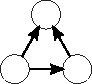
\includegraphics[width=\fig1width]{ttriad.pdf} & Transitive Triad (Balance)\linebreak[4]$\sum_{i\neq j\neq k}y_{ij}y_{jk}y_{ik}$  \\

\includegraphics[width=\fig1width]{homophily.pdf} & Homophily\linebreak[4]$\sum_{i\neq j}y_{ij}\mathbf{1}\left(x_i=x_j\right)$ \\
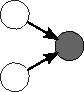
\includegraphics[width=\fig1width]{nodeicov.pdf} & Covariate Effect for Incoming Ties\linebreak[4]$\sum_{i\neq j}y_{ij}x_j$ \\
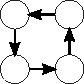
\includegraphics[width=\fig1width]{fourcycle.pdf} & Four Cycle\linebreak[4]$\sum_{i\neq j \neq k \neq l}y_{ij}y_{jk}y_{kl}y_{li}$  \\
\bottomrule
\end{tabular}
\caption{\label{fig:ergm-structs}Besides of the common edge count statistic (number of ties in a graph), ERGMs allow measuring other more complex structures that can be captured as sufficient statistics. }
\end{figure}

Although ``small networks'' is a topic mentioned several times in the literature on social network models  \cite{Wasserman1996,Frank1986,Snijders2011},  interest in larger social networks has dominated the field.\footnote{This is perhaps because, as put by \cite{Snijders2011}, small networks are considered to be ``uninteresting special cases''} Thus, ERGM methods have been developed to accommodate larger networks (although they do not scale well to ``very large'' networks of several thousand nodes or more). One example of this is the calculation of the likelihood function: rather than being calculated using exhaustive enumeration (which we will refer to as "exact likelihood"), the most popular software packages used for estimating these models apply simulation-based estimation methods. As a consequence, current methods used to estimate ERGMs for medium to large networks do not translate well to small network data (i.e., 10 or fewer nodes), and applications of these statistical network models to small networks are rare.  

One major technical and theoretical issue in ERGM estimation generally, which is exacerbated with small networks, is the problem of \textit{degeneracy}. Degenerate models occur when the observed graph statistics lie in a region on or near the boundary of the support, and can be stressed when estimation depends on Monte Carlo Integration \cite{Strauss1986,Handcock2003}. Small networks, which are more likely to be nearly empty or nearly full, have a smaller region of support, and are more likely to be on or near the boundary of that support. For example, if we are trying to estimate an ERGM in a network with only three nodes, in the scenario where the graph is directed and does not allow for self-ties, the chances of obtaining a graph with either one or zero ties (i.e., empty or almost completely empty), or a graph with five or six ties (i.e., fully or almost fully connected) is about 20\% using a uniform sampler. The degeneracy problem is so common with small networks (e.g., three to ten nodes). 

Because researchers studying small networks often have observed \textit{samples} of small networks (e.g., multiple team, family, or personal/egocentric networks), a common work-around to the issue of model degeneracy is to combine the independent small networks into a single larger block-diagonal graph. Estimation then proceeds by assuming that ties between blocks are impossible (i.e., treated as structural zeros in estimation). The major problems with this approach are that it can be complicated to fit, and difficult to extend. For example, the same set of constraints (the structural zeros) that allows for the model to be fit can also make the estimation procedure more difficult, and increase the possibility of sampling problems during MCMC estimation. More importantly, however, the block-diagonal approach can be difficult to extend. For example, a basic "complete pooling" model that assumes a common data generating process across all networks is straightforward to define using existing tools for ERGM estimation. However, relaxing that assumption to allow for variability across graphs (i.e., an unpooled model) can become problematic; this would typically require the creation of block-wise node membership attributes, and complex interaction terms involving subgraph statistics and node membership variables. Moreover, extending such a framework to not just allow for between-group variability, but to \textit{predict} it (for example, as a function of additional group-level variables), is not straightforward in such an approach.

To overcome the challenges described above for fitting ERGMs to small networks, we leverage the fact that in the case of small networks, the full likelihood function \textit{is} tractable. This allows the direct estimation of model parameters without using Markov Chain Monte Carlo (MCMC) or other approximate methods, avoiding some of the convergence issues associated with inference degeneracy \cite{Handcock2003}. It also opens up the possibility of making it much easier to combine ERGMs with other statistical techniques, opening the door for richer methods for modeling and understanding small-group structure and dynamics. In this paper, we describe how modern computational power allows for the complete specification of the likelihood for small graphs, and how this specification allows us to use the standard tools of maximum likelihood estimation (MLE), as opposed to approximate methods, including confidence intervals and likelihood ratio tests. We present examples using these techniques, provide some initial Monte Carlo results on bias, type I error rates, and power, and discuss future extensions these techniques make feasible.

\section{\ergmitos{}: ERGMs for small networks}

With modern computers, calculating the exact likelihood function of an ERGM for a small network becomes computationally feasible. This has an important implication: the process for estimating the parameters of an ERGM for small networks can be done directly. Many innovative techniques have been developed to handle models with intractable normalizing constants (e.g., MCMC-MLE, Bayesian techniques such as the exchange sampler, etc.), and often these techniques work quite well. Of course, no techniques are without tradeoffs; MCMC-MLE estimation can be very sensitive to starting values, and the quality of standard errors can depend on the availability of analytic gradients \cite{Park2018}. Bayesian techniques like the exchange sampler \cite{Moller2006} may be comparatively slow, which may be an issue when many networks are to be analyzed.

Moreover, simulation-based methods may have particular susceptibilities to model degeneracy. As stated by \cite[p. 7]{Handcock2003}, "[i]f the model used to simulate the graphs is not close enough to produce realizations that cover the observed values of the statistics, the MC-MLE will not exist even in cases where the MLE does." For example, many common network models, such as triangle-based models, can lead to bimodal distributions of graph statistics that simulation-based methods have difficulty with, even when the MLE falls between the modes \cite{Hunteretal2012}. Therefore, even though the degeneracy issue is not completely avoided, a method based on exact (non-simulation) inference may not only provide a better solution (in general) by avoiding the additional uncertainty induced by simulations and approximations, but may help mitigate the degeneracy issue in cases where the MLE exists.

Of course, the statistical analysis of a single small network is going to be uninformative due to the small numbers of dyads, and a high restriction in the variability of possible subgraph statistics. Fortunately, small network data is typically collected from \textit{samples} of small groups, which allows for the development of models to analyze structural variation both within and across small networks. If we assume that the sample of networks comes from a population of networks (groups) that are governed by the same data generating process, we end up with the following likelihood, defining a completely-pooled model:

\begin{equation}
    \label{eq:ergm-pooled}
    \Prcond{\Adjmat_1 = \adjmat_1, \dots, \Adjmat_P = \adjmat_P}{\params, \Indepvar_1, \dots, \Indepvar_p} = \prod_{p=1}^P\frac{%
    		\exp{\transpose{\params}\sufstats{\adjmat_p, \Indepvar_p}}%	
    	}{
    		\kappa_p\left(\params, \Indepvar_p\right)
    	}
\end{equation}

\noindent Where $P$ denotes the number of networks used in the model, and $\kappa_p\left(\params, \Indepvar_p\right)$ is explicitly calculated, unlike existing approaches to ERGM estimation. We call this framework, which is a revisited version of ERGM in the case of small networks, \ergmito{}\footnote{The \textit{ito}/\textit{ita} suffix is used in Spanish to denote small, or affection. We are especially grateful to George Barnett who proposed the name during the North American Social Networks Conference in 2018.}.

One complication with ERGMs involving multiple networks is that such models are usually not projective \cite{shalizi2013}, and the magnitude of parameter estimates and their standard errors (at least with network statistics in standard use) are all implicitly conditioned on network size. This means caution is required when combining (or comparing) parameter estimates from different networks. Even the interpretation of the basic edge count parameter can become difficult; as pointed out in \cite{Krivitsky2011}, assuming a common edge parameter in networks of different sizes is equivalent to assuming equal edge probabilities (verify this doesn't need qualification, e.g., conditional probs). This implies that one assumes network density increases as network size increases, but many real-world social networks are sparse and density grows much more slowly than network size. 

This is a significant concern in cases where samples of networks may span a wide range of sizes, and requires careful consideration of issues regarding choice of network statistics and the appropriateness of a completely-pooled approach (compared to, for example, a partially-pooled approach that allows for variability in estimates across networks). However, in the case outlined in this paper we focus on a sample of networks that are of similar size, and we assume there is a common data-generating process. The requirements and assumptions of the completely-pooled model in \eqref{eq:ergm-pooled} therefore can be assumed to hold. 

The simulations and model fitting were conducted using the R package \texttt{ergmito}, which has been developed to implement the methods described in this paper.

\section{Illustration with simulated data: fivenets}

\subsection{Data-generating-process and model fitting}

In the following section we work with a simulated data set that was created using the data-generating-process of \ergmitos{}. This particular dataset, which we call ``fivenets'', is included in the in the R package \texttt{ergmito}\footnote{The R package is available to be downloaded at  \url{https://github.com/muriteams/ergmito}.}. The data set contains five simulated networks with nodal attributes (we use gender in the following example), and the networks were generated using the following specification:

\begin{multline*}
\Prcond{\Adjmat = \adjmat}{\Indepvar_{\mbox{gender}}, \params} = \\
\frac{ %
    \exp{\params_{edges}\left(\sum_{i,j} \adjmat_{ij}\right) + %
    \params_{homophily}\left(\sum_{i,j} \adjmat_{ij}\isone{\Indepvar_{gender, i} = \Indepvar_{gender, j}}}\right) %
    }{%
    \normconst{}
    }
\end{multline*}

\noindent where $\params_{edges} = -2.0$ and $\params_{homophily} = 2$. Using this equation we draw five networks of size five. The process of ``homophily'' is represented by a parameter that is defined as the number of ties in which ego and alter have the same gender. Before drawing the networks we randomly generated the node attribute (gender) parameter to each vertex as a Bernoulli with parameter 0.5. \autoref{fig:fivenets} shows the generated networks, including their nodal attributes.

\begin{figure}[tb]
    \centering
    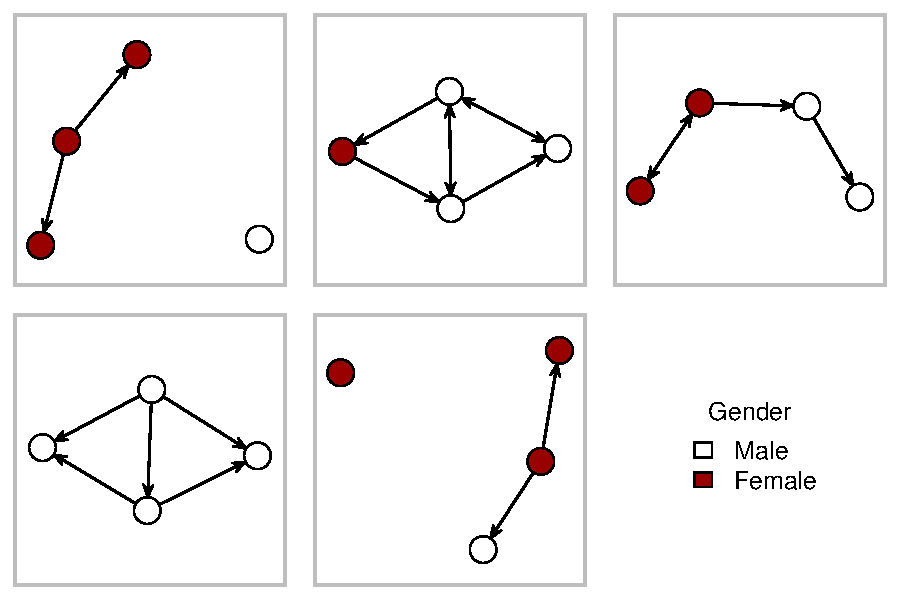
\includegraphics[width=.6\linewidth]{fivenets_graphs.pdf}
    \caption{\label{fig:fivenets}Fivenets data set. These graphs were randomly drawn from an ERGM distribution with two parameters: number of edges and gender homophily, with parameters equal to -2.0 and 2.0 respectively.}
    \label{fig:my_label}
\end{figure}

Using the \texttt{ergmito} R package, we fit three different models to the data\footnote{Some details regarding the computational aspects of the model fitting process are provided in \ref{appendix:mle}.}: (1) a Bernoulli graph, which is a model that only includes the ``edges'' parameter, (2) a model with ``gender homophily'' as its only parameter, and finally (3) a model including both ``edges'' and ``gender homophily'', this is, the correct specification of the model. \autoref{table:coefficients} shows the estimation results of the three different specifications of the model and as expected, model (3) has the best overall fit to the data. Furthermore, since all three models were fitted using MLE, we can compare the edgecount and homophily models with the full model using Likelihood Ratio tests \cite{Zeileis2002}. The \textit{goodness of fit} of this model is evaluated in the following section.


\begin{table}
\begin{center}
\begin{tabular}{l c c c }
\hline
 & Homopholy & Edgecount & Full model \\
\hline
Edgecount             &          & $-0.69^{*}$ & $-1.70^{**}$ \\
                      &          & $(0.27)$    & $(0.54)$     \\
Homophily (on Gender) & $-0.12$  &             & $1.59^{*}$   \\
                      & $(0.34)$ &             & $(0.64)$     \\
\hline
AIC                   & 85.06    & 78.38       & 73.34        \\
BIC                   & 87.15    & 80.48       & 77.53        \\
Log Likelihood        & -41.53   & -38.19      & -34.67       \\
Num. networks         & 5        & 5           & 5            \\
\hline
\multicolumn{4}{l}{\scriptsize{$^{***}p<0.001$, $^{**}p<0.01$, $^*p<0.05$}}
\end{tabular}
\caption{Fitted ERGMitos using the fivenets dataset. As expected, the Full model (last column of the table) has overall a better fit of the data. More over, the 95\% level CI of each covers the true parameters: $\hat\theta_{edges} \in [-2.77, -0.64]$; $\hat\theta_{Homophily} \in [0.33, 2.85]$.}
\label{table:coefficients}
\end{center}
\end{table}



\subsection{Goodness-of-fit in \ergmitos}

Researchers that apply ERGMs should be familiar with the goodness-of-fit (GOF) diagnostics that are used to assess how well the estimated model can reproduce graphs that are similar to the observed graph on a range of local and global graph statistics \cite{Hunteretal2008}. In the case of \ergmitos{} applied to small networks, local graph statistics will be more relevant than global statistics to assess GOF. For example, the graph geodesic distribution (i.e., the distribution of shortest-path lengths) is often used to assess GOF for larger networks, but this is clearly less relevant in the case of small networks (less than 10 nodes) because the shortest-path length between any two nodes typically lies between 1 and 2 steps. Therefore, we focus the GOF analysis on the parameters fit in the model as the bare-minimum of local graph statistics, as shown in \autoref{fig:fivenets-gof}. An important difference in our approach compared to traditional GOF assessments for ERGMs is that we are able to enumerate the full support of the model, and so instead of showing a boxplot we present a 90\% exact confidence interval per-statistic per network, comparing the fitted model's distribution with the observed parameters. A detailed discussion of this aspect of the \ergmitos{} is presented at the end of this paper.

\begin{figure}[tb]
    \centering
    \caption{Goodness-of-fit in \ergmitos{}. This illustrates how the observed sufficient statistics of each one of the 5 networks (x-axis) locate in the overall estimated distribution based on the fitted \ergmito{}. The gray lines in each box show the minimum and maximum value that the sufficient statistics can take in each one of the 5 networks, whereas the dotted lines provide a 90\% confidence interval. The dots are the observed statistics in each network.}
    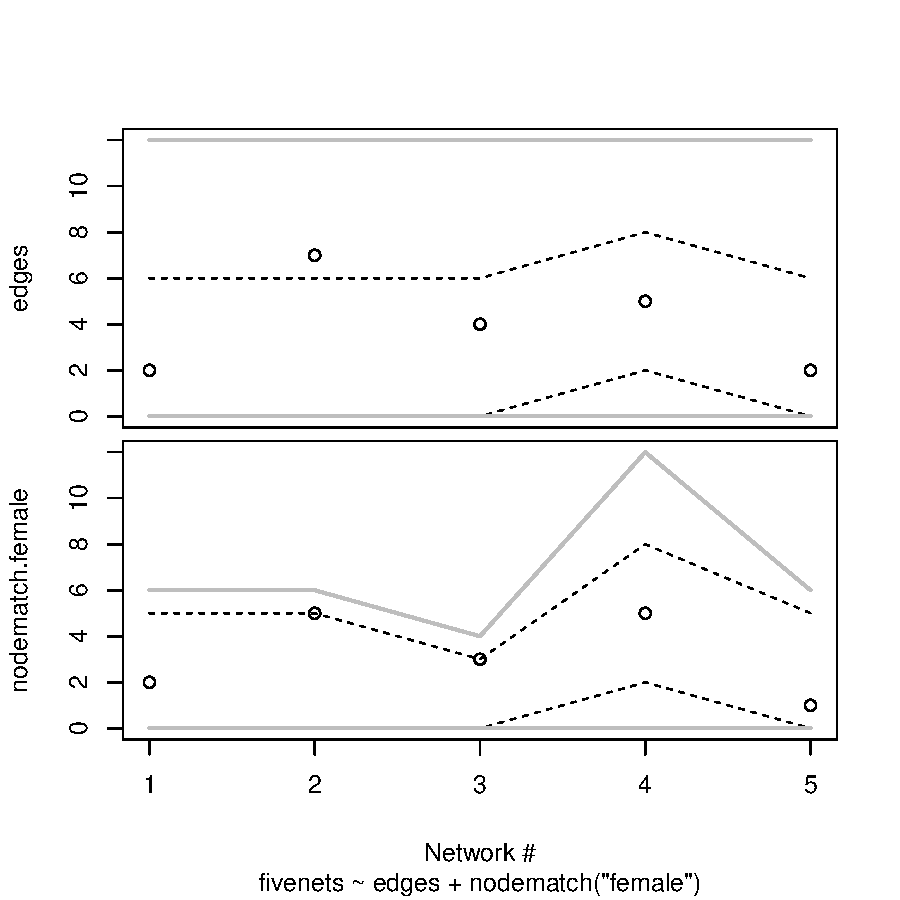
\includegraphics[width=.7\linewidth]{fivenets_gof.pdf}
    \label{fig:fivenets-gof}
\end{figure}

An important advantage of the \ergmitos{} over ``regular'' ERGMs is that we can observe the surface of the log-likelihood over different combinations of parameters in a rather straightforward way. This, together with the GOF analysis should be a routine step done after every \ergmito{} fit. \autoref{fig:fivenets-loglike} shows the surface of the log-likelihood function around the solution parameters to the maximization problem.

\begin{figure}[tb]
    \centering
    \caption{Surface of the log-likelihood function of the pooled \ergmito{} model. Lighter colors represent higher values while darker ones represent lower values. The red dot corresponds to the location of the MLE estimate of the model.}
    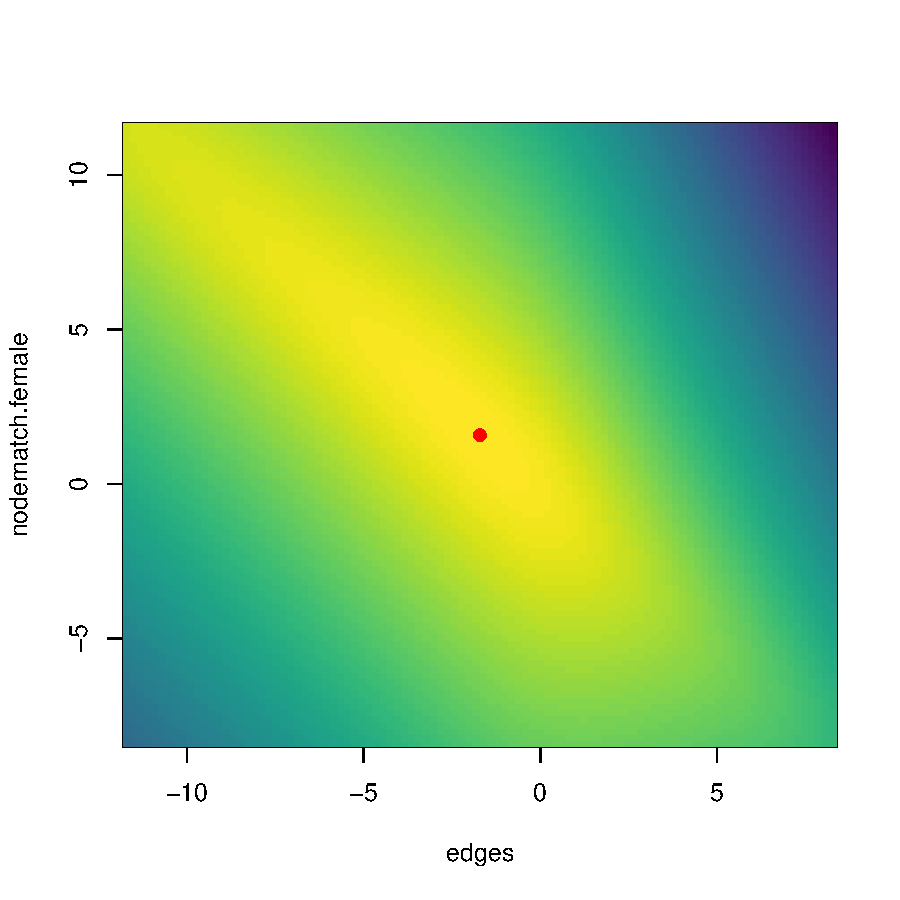
\includegraphics[width=.7\linewidth]{fivenets_loglike.pdf}
    \label{fig:fivenets-loglike}
\end{figure}

The ability to calculate the surface of the exact likelihood function, allows us to assess the quality of the estimated set of parameters. One good use of this diagnostic is to evaluate the roughness of the log-likelihood function, which in principle should give us an idea of the likelihood of the maximization process failing to reach a global maxima.

\pagebreak
\section{Simulation study}

We conducted two sets of simulations studies in which we compare the performance of MLE with MC-MLE in terms of bias, power, and type I error rates. In the first set, we analyze empirical bias and empirical power of each estimator in an scenario in which the ERGM is defined by \textit{edgecounts} and \textit{transitive triads}. For the second set of simulations, we look at empirical type I error rates when ERGMs are misspecified by including a \textit{transitive triad} term in the context of a data-generating-process that only includes an \textit{edgecount} statistic.

The code used to reproduce this entire section can be found at \url{https://github.com/muriteams/ergmito-simulations}.

\subsection{\label{subsec:design}Empirical Bias and Power}

Using the \ergmito{} R package, we generated 20,000 samples (datasets) consisting of several small networks. Each sample was generated using different combinations of parameters. While all come from an ERGM model defined by edgecounts and number of transitive triads, for every sample we specified: (1) population parameters for the ERGM, (2) size of the sample (number of networks in the sample), and (3) composition of the sample in terms of the combination of networks of size four and five. A detailed description of each one of these three components used to draw the samples follows:

\begin{enumerate}
\item \textbf{Population parameters} First we drew two numbers from a piece-wise Uniform distribution with values in $[-2, -.1]\cup[.1, 2]$, ($\params_{edges}, \params_{ttriads}$), which corresponded to the parameters associated to the statistics \textbf{edgecount} and \textbf{number of transitive triads}. This specifies the ERGM from which we will be drawing the networks from. This is akin to \cite{Schweinberger2015} approach to simulate ERGM from outside of degenerate areas, although we took a more conservative approach than their ranges of (-5,0) and (0, 5) for the parameters ``edges'' and ``triangles'' in order to increase the number of non-degenerate samples, this is, samples composed mostly by either empty of fully connected graphs.

\item \textbf{Number of networks per sample} Then, we specified the number of networks to generate from the model defined in the previous step, using one of the following sample sizes $\{5, 10, 30, 50, 100, 150, 200, 300\}$. Notice that overall, for each one of the possible set of sample sizes, we ended up generating 2,500 samples for each sample size, in other words, we generated 2,500 samples with 5 networks, 2,500 samples with 10 networks, etc.

\item \textbf{Number of nodes per network} Finally, the composition of each sample in terms of the number of vertices that each network has was uniformly-random selected from the pairs $\{N, 0\}, \{N - 1, 1\}, \dots, \{1, N - 1\}, \{0, N\}$, where the first number of each pair is the number of networks of size 4, and the second is the number of networks of size 5 in the sample, for example, if the sample size selected in the previous step was 30, then the possible pairs to select from would be $\{30, 0\}, \{29, 1\}, \dots, \{1, 29\}, \{0, 30\}$, so samples in which all networks were of size 4 (meaning we draw the pair $\{30, 0\})$ or size 5 (again, selecting the pair  $\{0, 30\}$) were equally likely. 
\end{enumerate}

For each one of the 20,000 simulated datasets, we then estimated the model using both MLE--as implemented in the \ergmito{} R package \cite{vegayon2018}--and MC-MLE--using statnet's \texttt{ergm} R package \cite{Handcock2018,hunter2008}. In the case of the latter, the pooled estimation was done by fitting what is know in the literature as a block-diagonal model in which (a) networks are stacked together in a single adjacency matrix, and (b) the sampling space for the MCMC process is constrained to sample from graphs where ties are only possible within blocks. We set the MCMC control parameters \textit{interval} and \textit{samplesize} to 2,048 (double the default values) to increase precision of the parameter estimates.

\subsubsection{Empirical Bias and Power: Samples in which either of MC-MLE or MLE returned with an error}

Of the models fit to the 20,000 datasets (each comprised of samples of small networks), in 14,963 cases the models were successfully fit using both the MLE and MC-MLE estimators. In 121 cases both implementations failed with an error, and for the remaining cases (4916) the MC-MLE (ERGM) failed in most of them (4905 of 4916), while implementation of the MLE (ERGMito) estimator failed in only 14 of these 4916 cases. Of the 4905 cases in which the MC-MLE failed, MLE was able to detect a significant effect in both parameters in 697 cases (i.e., 14 percent of these cases). Conversely, of the 14 cases in which the MLE failed, MC-MLE was not able detect a significant effect in any of these cases.. \autoref{fig:failed-tree} summarizes the succesful and failed models described above.

\begin{figure}
	\centering
	\caption{\label{fig:failed-tree}Distribution of the failed estimations. A failed estimation attempt refers to the case in which the implementation of the algorithm (ERGM for the MC-MLE, and ERGMito for the MLE method), returned with an error.}
	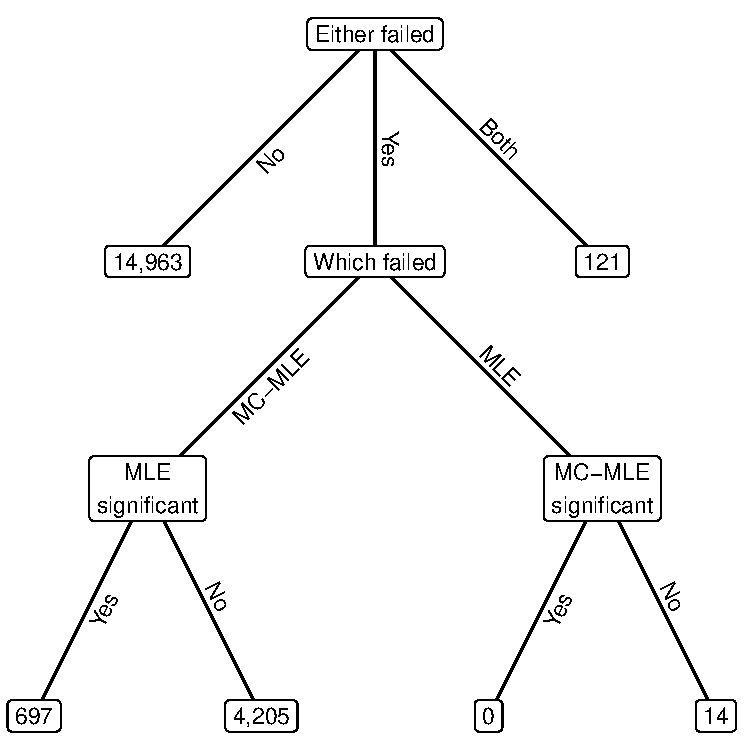
\includegraphics[width=.5\linewidth]{failed-tree.pdf}
\end{figure}

To gain insight into the problems causing the failed models, we considered the distribution of the sufficient statistics. These indicate that most of the problems arose in situations where the sufficient statistics were near to the boundary of the support. This is illustrated in \autoref{fig:failed}, and shows that in most of the cases in which both methods failed, the sufficient statistics were mostly saturated, meaning they reached the maximum possible value because the  cases sampled were largely composed of fully connected networks. Given errors arose when the set of sufficient statistics was close to saturation, both ERGM and ERGMito should consider those cases and test for possible failures during the estimation process.

\begin{figure}
	\centering
	\caption{\label{fig:failed}Distribution of the average sufficient statistics per sample. Since samples can contain networks of sizes four and five, we have re-scaled the sufficient statistics counts by each network size's corresponding maximum value so these range from zero to one.}
	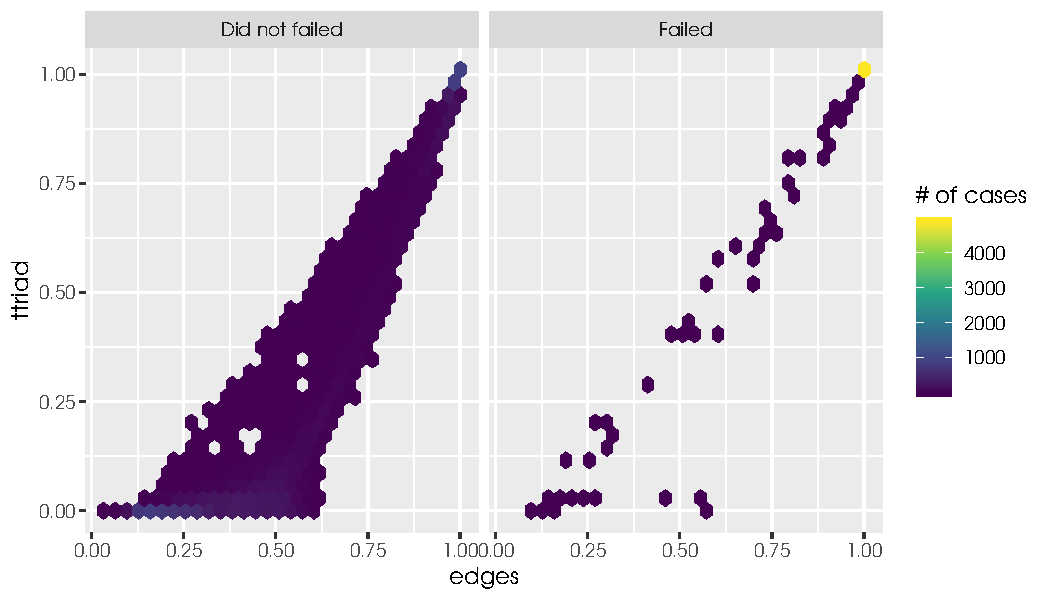
\includegraphics[width=.8\linewidth]{failed.pdf}
\end{figure}

We also considered if the rate of model failure was greater when the dataset contained a smaller sized sample of networks. \autoref{tab:error-sampsize} shows the error rates by sample size for both implementation methods, and it is clearly higher for smaller samples (particularly less than 30 networks), and this is especially true for MC-MLE. 

Moreover, if the optimization algorithms are able to return anything, both ERGM and ERGMito try to compute variance-covariance matrices using the model's log-likelihood; this being approximated in the case of MC-MLE. It is important to note that in the case that the Hessian matrix is not p.s.d (positive-semi-definite), both ERGM and ERGMito use the Moore-Penrose generalized inverse algorithm as implemented in the R package MASS \cite{Venables2002}. For more on the interpretation of variance-covariance matrices when the Hessian is not p.s.d., see \cite{Gill2004}. Details on the evaluation of parameter estimates in ERGMIito can be found in \autoref{sec:evaluation-of-estimates}.

% latex table generated in R 3.6.1 by xtable 1.8-4 package
% Wed Sep 11 15:07:30 2019
\begin{table}[ht]
	\centering
	\begin{tabular}{lcc}
		\toprule & \multicolumn{2}{c}{P(Error)} \\ \cmidrule(r){2-3}
		Sample size & MC-MLE & MLE \\ 
		\midrule
		5 & 0.35 & 0.00 \\ 
		10 & 0.32 & 0.03 \\ 
		30 & 0.27 & 0.01 \\ 
		50 & 0.25 & 0.01 \\ 
		100 & 0.23 & 0.00 \\ 
		150 & 0.20 & 0.00 \\ 
		200 & 0.20 & 0.00 \\ 
		300 & 0.18 & 0.00 \\ 
		\bottomrule
	\end{tabular}
	\caption{\label{tab:error-sampsize}Failure probability (software implementation) by sample size.} 
\end{table}


Finally, it is important to highlight that unexpected errors during the estimation process, despite being associated with properties of each estimation method, are issues that could be resolved through software development and so can be improved.

\pagebreak

\subsubsection{Empirical Bias and Power: Samples fitted successfully}

Out of the 20,000 model fitting attempts on the simulated datasets, about 25\% of those fit with either MLE or MC-MLE failed to return an estimate. The results that follow only include those samples in which both MLE and MC-MLE methods returned without an error. As shown in \autoref{fig:bias}, both estimation methods behaved similarly in terms of empirical bias in the models studied here. As the size of the sample of networks in the dataset increased (i.e., when there were more networks within the sample), the empirical bias of both MC-MLE and MLE decreased, as expected.

\begin{figure}
	\centering
	\caption{\label{fig:bias}Empirical distribution of the bias per model parameter, for MC-MLE and MLE estimation methods. In general we see that the parameter estimates' bias is centered around zero and both MC-MLE (ERGM) and MLE (ERGMito) have about the same bias in our simulation study.}
	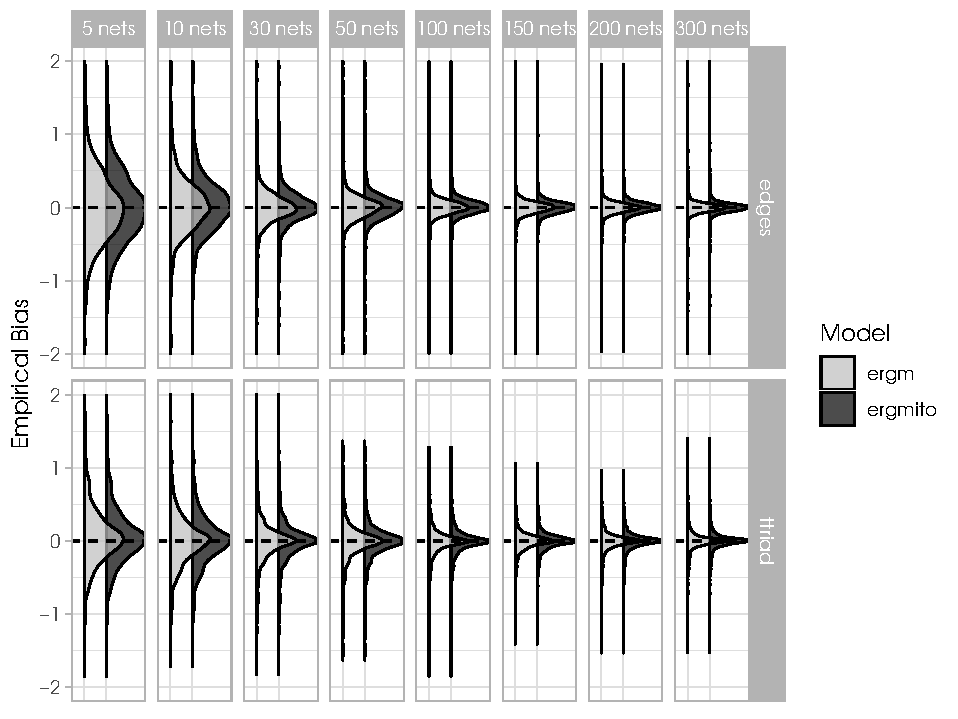
\includegraphics[width=.8\linewidth]{bias-02-various-sizes-4-5-ttriad.pdf}
\end{figure}

As shown in \autoref{fig:power}, both MC-MLE and MLE behave very similarly with empirical power levels increasing as the size of the sample of networks increases in the dataset size (the x-axis of each sub-figure), and as the effect size increases (the y-axis of each sub-figure). Moreover, we compared power levels using two-sample proportion tests and found no significant differences between the power levels of MC-MLE and MLE. It is interesting to note that, in the case of effect sizes of magnitude [0.5, 1.0), the discovery rate for the \texttt{ttriad} parameter reaches nearby 0.75 for sample sizes between 30 to 50 networks, which is a rather common sample size in the study of small networks such as teams, families, and sometimes ego-networks. 

\autoref{fig:power-prop5s} shows the effect of the composition of the sample in each dataset, in terms of the proportion of networks of size five (vs. size four), and the number of networks per dataset. In this case, we observe no meaningful patterns that would indicate the dataset composition is related to power.

\begin{figure}[ht]
	\centering
	\caption{\label{fig:power}Empirical power by dataset size and effect size (the later considering only magnitude), for ERGM and \ergmito{} estimation methods. Power increases for both MC-MLE (ERGM) and MLE (\ergmito{}) with increases in the size of the dataset and effect size. There are indistinguishable differences in power between the two estimation methods.}
	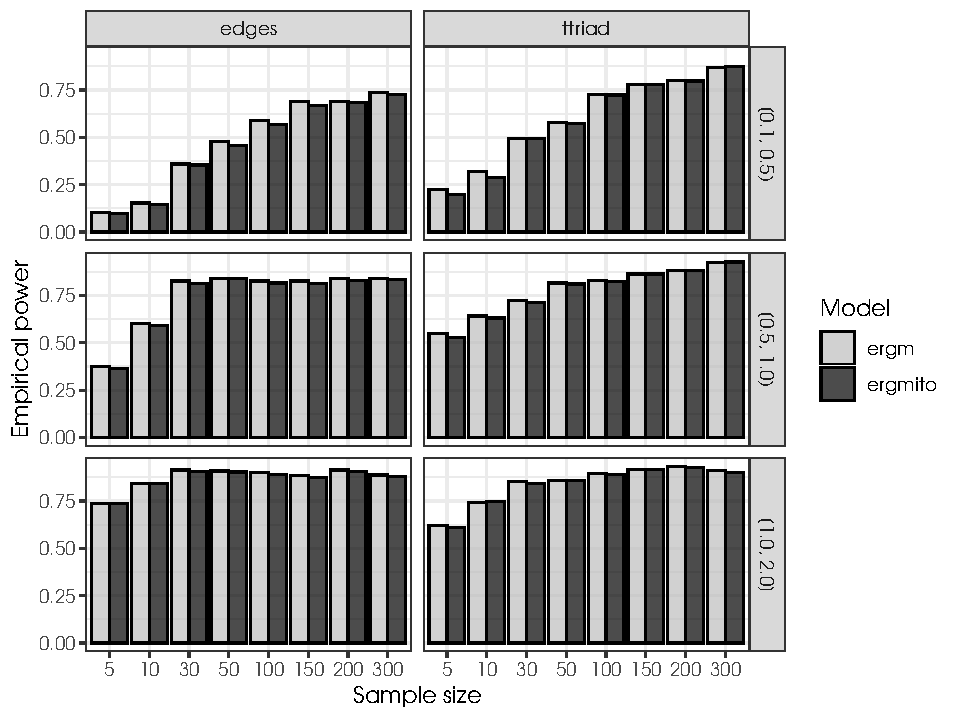
\includegraphics[width=.9\linewidth]{power-by-model.pdf}
\end{figure}

\begin{figure}[ht]
	\centering
	\caption{\label{fig:power-prop5s}Empirical power by proportion of networks of size five in the sample (color coded) and sample size (rows).}
	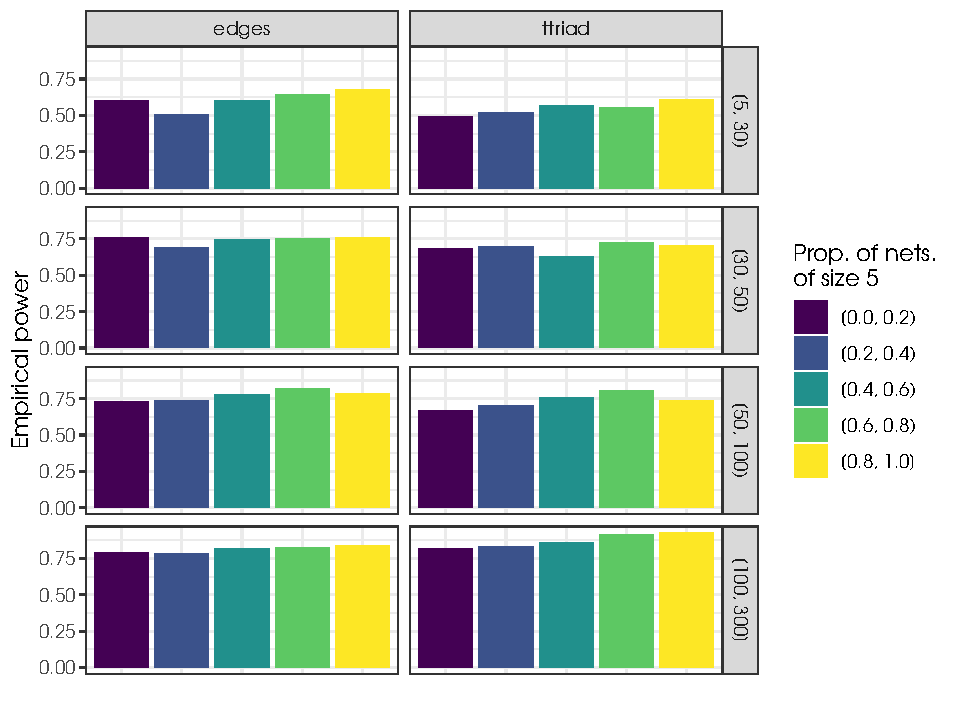
\includegraphics[width=.7\linewidth]{power-by-prop-of-fives.pdf}
\end{figure}

One notable difference between the two estimation methods was in computational time: using MLE makes the estimation process significantly faster. As shown in \autoref{fig:elapsedtime}, MLE (\ergmito{}) is orders of magnitude faster than MC-MLE (ERGM). Therefore, while both estimators show very similar properties in terms of power and bias, practitioners will benefit by using MLE (\ergmito{}) when modeling small networks because it may substantially reduce the estimation time.\footnote{While this is mostly true, there are some scenarios in which the speed gains may not be as dramatic as it has been showed here. The biggest computational bottleneck that \ergmito{} faces is the calculation of the full support of the sufficient statistics. In the case of structure-only statistics, \ergmito{}, and actually \textit{ergm}, computes the full distribution very quickly, but, as the model starts to become more complex, such calculation becomes more expensive.}

\begin{figure}
	\centering
	\caption{\label{fig:elapsedtime}Distribution of elapsed time (in seconds) for the estimation process for MC-MLE (ERGM) versus MLE (using \ergmito{}). Overall, the MLE implementation is orders of magnitude faster compared to the time required by the MC-MLE implementation to do the parameter estimation.}
	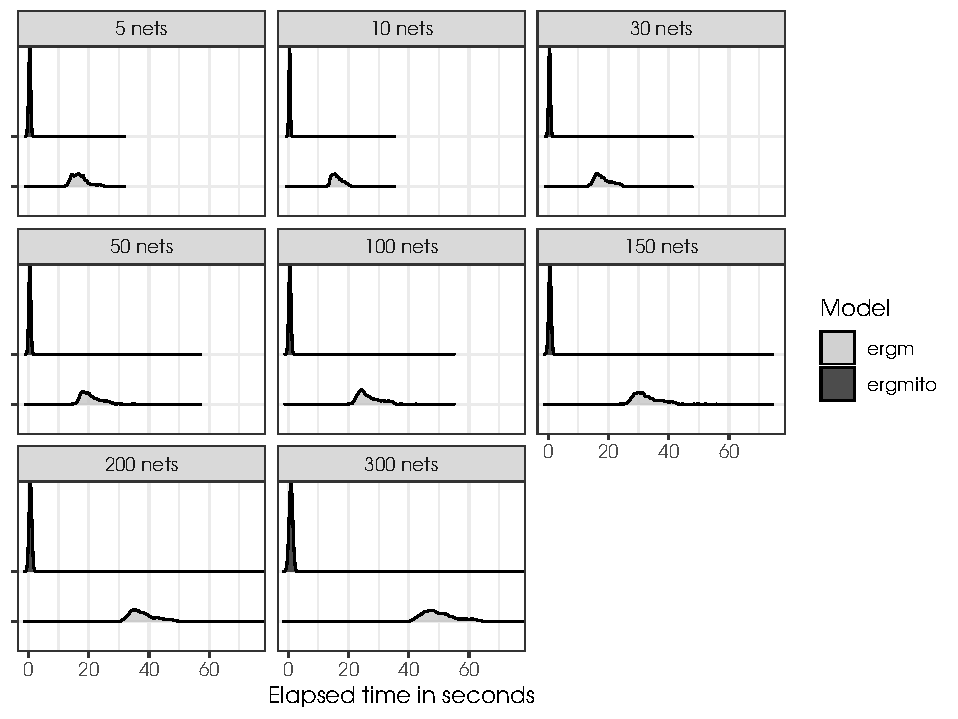
\includegraphics[width=.9\linewidth]{bias-elapsed-02-various-sizes-4-5-ttriad.pdf}
\end{figure}





\subsection{Type I error rates}

Using the same procedure described in \autoref{subsec:design}, we simulated 17,500 datasets comprised of Bernoulli networks (i.e., an ERGM model only defined by the \textit{edgecounts} sufficient statistic). In this case, we drew  different sets of sample sizes: for each of $\{5, 10, 15, 20, 30, 50, 100\}$ we generated 2,500 datasets using the Bernoulli model with \textit{edgecount} parameter uniformly distributed in the range $[-2, -.1]\cup [.1, 2]$. We then estimated the models using MC-MLE and MLE, as implemented in the ergm and ergmito R packages respectively, and calculated the type I error rates, using a misspecified model, this is, fitting ERGMs including a \textit{transitive triads} count statistic. 

As shown in table \autoref{tab:typeI}, when models are fit to datasets with samples sizes of 15 or less networks, the MLE estimates had a significantly smaller type I error rate at the 5\% significance level, after comparing both rates using a two-sample proportion test. With datasets that had samples sizes of 20 or more networks, there was no statistically significant difference in type 1 error rates between the two methods.

% latex table generated in R 3.6.1 by xtable 1.8-4 package
% Mon Sep  9 13:04:55 2019
\begin{table}[ht]
	\centering
	\begin{tabular}{ccccc}
		\toprule & & \multicolumn{2}{c}{P(Type I error)} \\ \cmidrule(r){3-4}
		Sample size & N. Simulations & MC-MLE & MLE & chi2 \\ 
		\midrule
		5 & 2,189 & 0.084 & 0.057 & 11.71 *** \\ 
		10 & 2,330 & 0.070 & 0.045 & 12.46 *** \\ 
		15 & 2,395 & 0.084 & 0.066 & 5.55 * \\ 
		20 & 2,430 & 0.074 & 0.060 & 3.58  \\ 
		30 & 2,460 & 0.057 & 0.052 & 0.67  \\ 
		50 & 2,495 & 0.046 & 0.044 & 0.17  \\ 
		100 & 2,499 & 0.048 & 0.048 & 0.00  \\ 
		\bottomrule
	\end{tabular}
	\caption{\label{tab:typeI}Empirical Type I error rates. The $\chi^2$ statistic is from a 2-sample test for equality of proportions, and the significance levels are given by *** $p < 0.001$, ** $p < 0.01$, and * $p < 0.05$. The lack of fitted samples in some levels is due to failure of the estimation method.} 
\end{table}



\pagebreak
\section{Discussion}

In this paper we revisit and extend Exponential Family Random Graph Models (ERGM) for the case of small networks. Given the interest in testing hypotheses about small networks in the literature, but limited application of statistical models to small network data, we proposed a special case of ERGMs for small networks, called \ergmitos{}. An appealing feature of \ergmitos{} is that the are estimated using MLE directly, rather than estimation via MCMC methods, as is traditionally done with ERGMs for larger networks. This approach provides a couple of important benefits for small network data: (1) it avoids at least partially, if not completely, the model near-degeneracy problems that affects the MC-MLE methods; and (2) its use of pooled estimates is valuable when datasets are comprised of small networks, as is often the case with research on multiple families, small teams, or ego-networks. Our simulation study finds that \ergmitos{} are easily estimated, and that this approach can improve accuracy and efficiency for modeling small networks compared to MC-MLE estimation approaches implemented in other ERGM pacakages.

Other topics to mention in discussion here: (1) full LL allows for simple extensions that are very difficult otherwise (use mixture model as example, perhaps mention hierarchical ERGMs since it's relevant to the model here and the general application space of team research); (2) if derivative is available and computeable, allows for advanced Bayesian methods like HMC, MALA, etc.

The development and evaluation of \ergmitos{} in this simulation study also brings up topics for future work. One is the evaluation of model goodness-of-fit, and identifying statistics that are most important to evaluate with small networks, and that are reasonable to expect in a model that would suggest a ``good fit''. Because \ergmitos{} enable a rather simple way of conducting simulation studies (relative to traditional ERGMs), this will facilitate this work in future. Another topic to explore in future work is the value of \ergmitos{} for estimating ERGMs for very large networks, by drawing \textit{samples} of local network structures from a large graph. There is ongoing work extending ERGMs to very large networks \cite{stivala2019exponential,STIVALA2016167}, and \ergmitos{} may be a valuable and \textit{efficient} approach for fitting these pooled models to a large sample (e.g., in the order of the thousands) of small local network structures, with 5 or 6 nodes, drawn from a large network. 

Overall,  \ergmitos{} provide a promising extension to the ERGM framework for the analysis of small social networks, which can generate a richer understanding of the local social processes that give rise to the formation of networks in small social groups, and processes that are the \textit{local social building blocks} of many larger social structures. 

\section{Acknowledgements}

This material is based upon work support by, or in part by, the U.S. Army Research Laboratory and the U.S. Army Research Office under grant number W911NF-15-1-0577. The views, opinions, and/or findings contained in this paper are those of the authors and shall not be construed as an official Department of the Army position, policy, or decision, unless so designated by other documents

Computation for the work described in this paper was supported by the University of Southern California’s Center for High-Performance Computing (hpcc.usc.edu).

\clearpage

\bibliographystyle{plain}
\nocite{VegaYon2019,R,butts2016,Wickham2016,Leifeld2013}
\bibliography{bibliography.bib}

\clearpage

\appendix

\section{MLE\label{appendix:mle}}

The estimation process of \ergmitos{} (as pooled models of small networks) is done entirely on R using the \texttt{ergmito} R package. While a significant amount of the implementation of the methods described here was done using \texttt{Rcpp} \cite{Eddelbuettel2011}, a core component of the package is based on statnet's \texttt{ergm} R package, and in particular, in the function \texttt{ergm.allstats} which does exhaustive enumeration of statistics in a compact way. In general, the estimation process for any list of networks is as follows:

\begin{enumerate}
    \item Analyze the model to be estimated: Extract the networks from the left-hand-side as specified in the ergm package, and calculate the exact statistics using the ergm.allstats function.
    \item With the full enumeration of statistics, build the joint likelihood function of the model in a compact form (i.e., using the weights instead of the full enumeration of the support of the model). This improves speed when it comes to evaluating the log-likelihood function.
    \item Because we are dealing with exact statistics, it is also possible to calculate the exact gradient function. We compute the gradient as follows:
    
    \begin{equation}
    \sum_{p}\nabla l_p(\theta) = \transpose{\sufstats{\adjmat_p, \Indepvar_p}} - \frac{\transpose{Q_p}\left(\transpose{W_p} \circ \exp{Q_p \theta}\right)}{\kappa_p}
    \end{equation}
    
    Where $\sufstats{\adjmat, \Indepvar}$ is a vector of observed sufficient statistics (usually called target statistics), $Q$ is a matrix of sufficient statistics, in particular, the isomorphic sufficient statistics associated with the model, and $W$ is a vector of frequency weights.
    
    These first three steps carry the most part of the computing time.
    
    \item Finally, the joint log-likelihood is maximized using the BFGS algorith implemented in the the optim function in the stats package.
    
\end{enumerate}

The final set of estimates is analyzed separately by another program included in the package. The next section describes the evaluation steps followed by \ergmito{}.

\section{\label{sec:evaluation-of-estimates}Evaluation of estimates}

After the optimization procedure finalizes, the \texttt{ergmito} package performs a series of tests checking the quality of the estimates. In particular, we conduct the following evaluations after every call to the main optimization function:

\begin{enumerate}
	\item Since the BFGS algorithm, as implemented in the \texttt{optim} function from the stats R package, only works with real numbers, we check whether the log-likelihood function increases with changes in the attained value in cases when the theoretical maxmima lies in $\pm\infty$. To do this, we increase the magnitude of each estimate by 1.5 and check the value of the log-likelihood function with that change. If an increase in that value is observed, we assume that the maxima for the given parameter equals $\mbox{sign}(\hat\theta_i)\times\infty$.
	
	\item If all parameters turn out to be $\pm\infty$ after this check, the function will send a warning message to the user and the function returns without computing the variance-covariance matrix.
	
	\item If, on the other hand, a fraction of the parameters were switched to $\pm\infty$, the function recalculates the Hessian and the log-likelihood using the value $\mbox{sign}(\hat \theta_i)\times 10^{5}$. This is done instead of using $\infty$, because in most cases using infinite will result in the function being undefined. Again, the function will warn users about this issue.
	
	\item Finally, using the current state of the Hessian matrix, the function will attempt to compute the variance-covariance matrix by inverting the negative of the Hessian. If an error is caught, then the generalized inverse is returned instead \cite{Gill2004}.
\end{enumerate}

The possible return codes are:

\begin{itemize}
\item[\textbf{00}] optim converged, no issues reported.
\item[\textbf{01}] optim converged, but the Hessian is not p.s.d.
\item[\textbf{10}] optim did not converged, but the estimates look OK.
\item[\textbf{11}] optim did not converged, and the Hessian is not p.s.d.
\item[\textbf{20}] A subset of the parameters estimates was replaced with +/-Inf.
\item[\textbf{21}] A subset of the parameters estimates was replaced with +/-Inf, and the Hessian matrix is not p.s.d.
\item[\textbf{30}] All parameters went to +/-Inf suggesting that the MLE may not exists.
\end{itemize}


\end{document}
